% Chapter 7
\chapter{Communication with LabVIEW User Interface using UART Port Controller} 
\label{Chapter7}
\lhead{Chapter 7. \emph{Communication with LabVIEW User Interface using UART Port Controller}}
\textsf{\textsl{Written by Thuy Pham}}
%----------------------------------------------------------------------------------------
\section{Introduction}
Communicating with peripheral devices plays a vital role in system design in general and in DSP systems specifically. For this purpose, SHARC Processor uses Digital Peripheral Interface (DPI). The interface provides both connections to two serial peripheral interface ports (SPI) and two universal asynchronous receiver-transmitters (UARTs). In this report, Universal asynchronous receiver transmitters (UARTs) will be examined in relationship with LabVIEW User Interface.\\
It is necessary to notice that the processor provide a full duplex universal asynchronous receiver/transmitter (UART) port, which is fully compatible with PC-standard UARTs. The UART port provides a simplified UART interface to other peripherals or hosts, supporting full duplex, DMA supported asynchronous transfers of serial data. The UART also has multiprocessor communication capability using 9-bit address detection. This allows it to be used in multi-drop networks through the RS-485 data interface standard. The UART port also includes support for five data bits to eight data bits, one stop bit or two stop bits, and none, even, or odd parity. More specifically, the UART port supports two modes of operation as mentioned below:
\begin{itemize}
\item \textbf{PIO (programmed I/O):} The processor sends or receives data by writing or reading I/O mapped UART registers. The data is double-buffered on both transmit and receive.
\item \textbf{DMA (direct memory access):} The DMA controller transfers both transmit and receive data. This reduces the number and frequency of interrupts required to transfer data to and from memory. The UART has two dedicated DMA channels, one for transmit and one for receive. This is the mode that will be used for transferring data between LabVIEW program and DSP board.
\end{itemize}
%----------------------------------------------------------------------------------------
\section{UART data frame}
\begin{figure}[htbp]
\centering
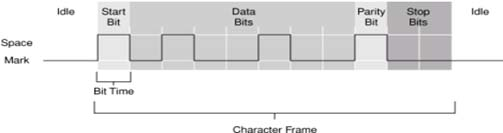
\includegraphics[height=3cm]{uart}
\rule{30em}{0.5pt}
\caption{A typical UART data frame}
\label{fig:uart}
\end{figure}
When two UARTs communicate, both transmitter and receiver need to know the signaling speed. The receiver does not know when a packet will be sent (no receiver clock); thus, the protocol is termed "asynchronous." This is very important because if we set up parameters (baud rate, start bit, stop bits, and parity bit) in both transmitter and receiver is incompatible, we will get incorrect data. In addition, the receiver circuitry is correspondingly more complex than that of the transmitter. The transmitter simply has to output a frame of data at a defined bit rate. Contrastingly, the receiver has to recognize the start of the frame to synchronize itself, and therefore determine the best data sampling point for the bit stream.\\ 
The processor supports a set of parameters' values for UART communication as below:
\begin{center}
\begin{tabular}[t]{|c|c|c|}
\hline
\textbf{SST} & \textbf{Parameters} & \textbf{Value}\\
\hline
1 & Baud rate & 2400, 4800, 9600, 19200, 38400, 57600, 115200, 921600, 6250000\\
\hline
2 & Data bits & 5 to 8 \\
\hline
3 & Stop bits & 1 or 2 \\
\hline
4 & Parity & None, even, odd \\
\hline
\end{tabular}
\end{center}
%----------------------------------------------------------------------------------------
\section{UART external interface}
The DSP processor communicates with peripheral devices in DSP board is described as the block diagram in figure \ref{fig:uart1}:
\begin{figure}[htbp]
\centering
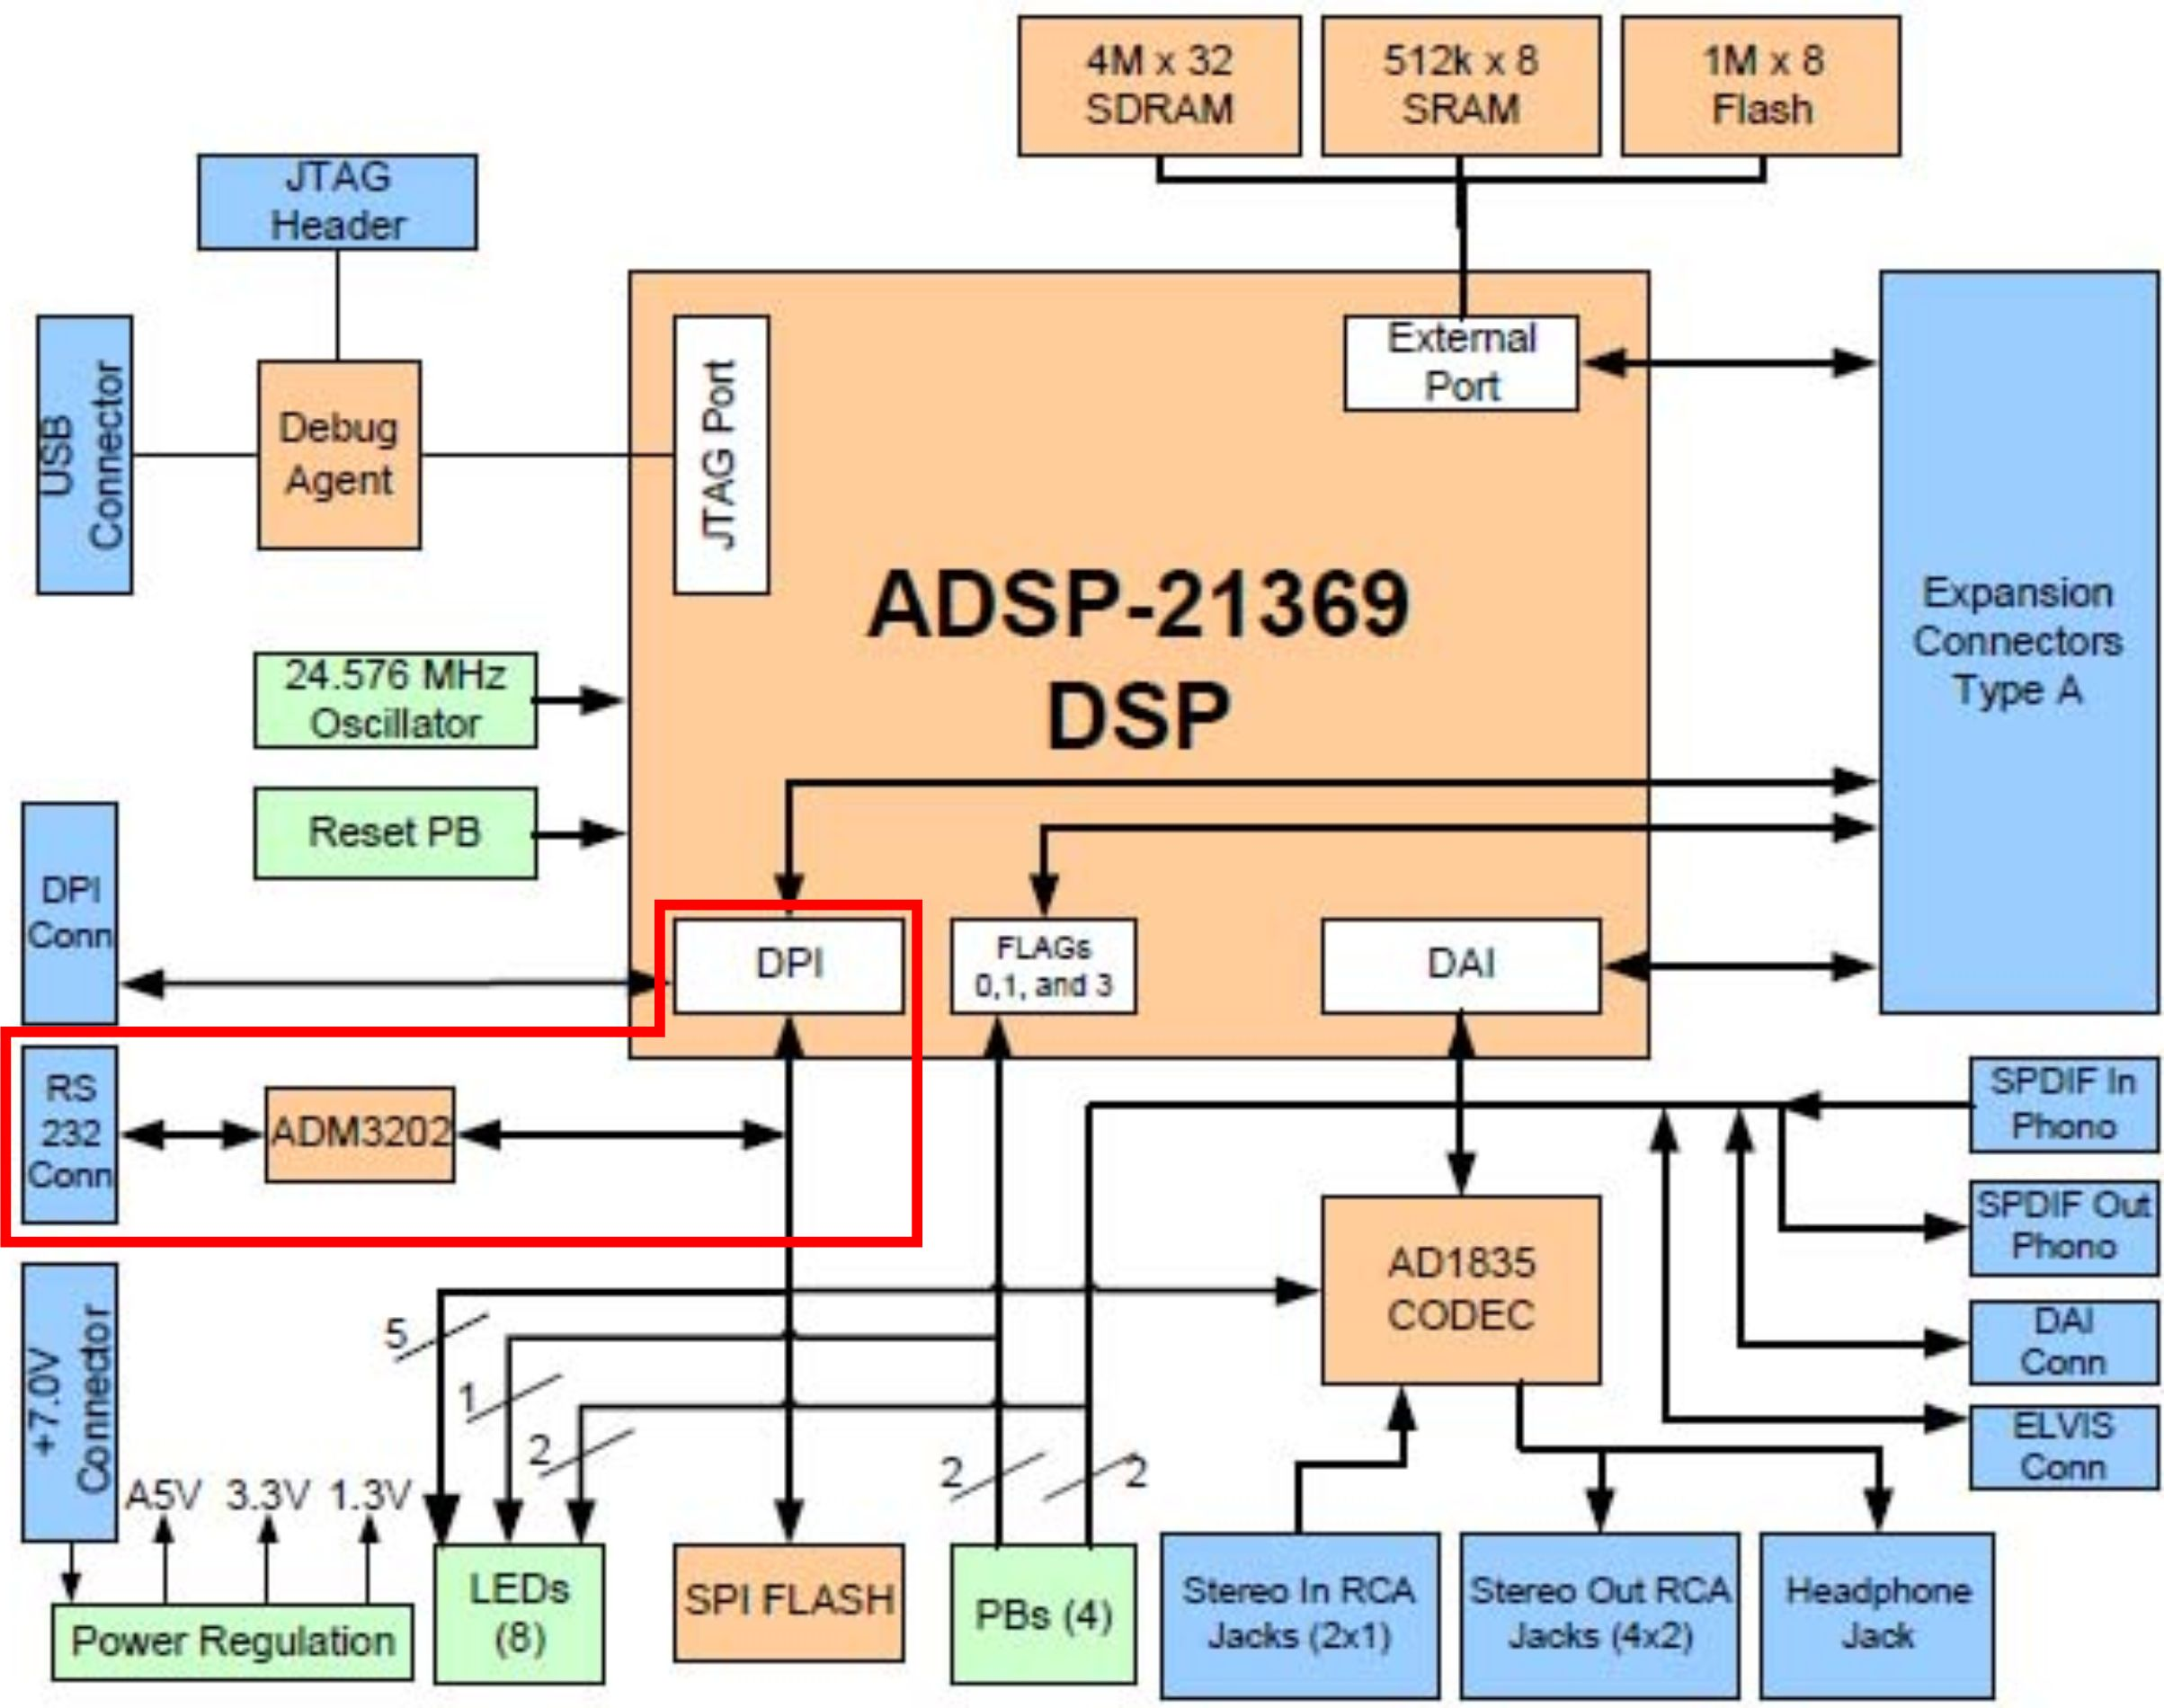
\includegraphics[height=8.5cm]{systemArchitectureDPI}
\rule{30em}{0.5pt}
\caption{System Architecture Block Diagram}
\label{fig:uart1}
\end{figure}\\
\begin{figure}[htbp]
\centering
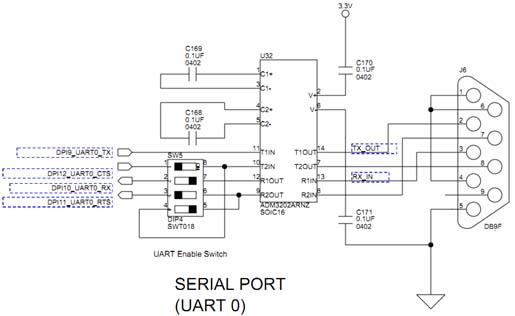
\includegraphics[height=6.5cm]{uart2}
\rule{30em}{0.5pt}
\caption{Schematic for connection of UART port}
\label{fig:uart2}
\end{figure}
In this board, the EIA-232E interface is used to communicate with other external serial communication devices. Instead of using traditional circuit for compatible purpose of power levels, in the DSP board, manufacture uses ADM3202 chip. The significant features of the chip are low power consumption and can operate at data rates up to 460 kbps make them ideal for battery powered portable instruments and high speed requirement.
%----------------------------------------------------------------------------------------
\section{UART configuration in DSP Processor for communication}
The DSP Processor provides a set of PC style, industry standard control and status registers for the UART.\\
\textbf{Register Overview for UART Module:}
\begin{itemize}
\item Line Control Register (UARTxLCR). Controls format of the data character frames. It selects word length, number of stop bits and parity.
\item Divisor Latch High/Low Register (UARTxDLL, UARTxDLH). Characterize the UART bit rate. The divisor is split into the divisor latch low byte (UARTxDLL) and the divisor latch high byte (UARTxDLH).
\item Mode Control Register (UARTxMODE). Controls packing and address modes.
\item Transmit Buffer Control Register (UARTxTXCTL). Controls core or DMA operation.
\item Receive Buffer Control Register (UARTxRXCTL). Controls core or DMA operation.
\item Interrupt Enable Control Register. Enables interrupt requests from system handling.
\item Line Status Register (UARTxLSR). Returns status of controls format of the data character frames as overrun or framing errors and break interrupts.
\item Transmit Status Register (UARTxTXSTAT). Returns status of core or DMA operations.
\item Receive Status Register (UARTxRXSTAT). Returns status of core or DMA operations.
\item Interrupt Identification Status Register (UARTxIIR). The register is used to get the status of all interrupts into one channel.
\end{itemize}
To configure parameters for transmitting data between PC and the DSP board, the number of simple steps can be followed:
\begin{enumerate}
\item \textbf{Route the UART to the DPI of DSP Processor}\\
The routing is implemented by software, in particular in the VisualDSP++, it is in the SRU macro. It is necessary to notice that, data is transmitted and received by the least significant bit (LSB) first (bit 0) followed by the most significant bits (MSBs).
\begin{figure}[htbp]
\centering
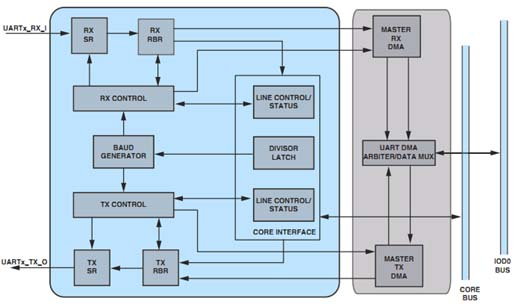
\includegraphics[height=6.5cm]{uart3}
\rule{30em}{0.5pt}
\caption{UART Functional Block Diagram}
\label{fig:uart3}
\end{figure}
\item \textbf{Set up baud rate, data bits, stop bits, parity bit}\\
The bit rate is characterized by the peripheral clock (PCLK) and the 16-bit divisor. The divisor is split into the UART divisor latch low byte register (UARTxDLL) and the UART divisor latch high byte register (UARTxDLH).  UART Baud rate = PCLK/(16 � divisor), where PCLK is the system clock frequency.\\
All data words require a start bit and at least one stop bit. With the optional parity bit, this creates a 7 to 12-bit range for each word. The format of received and transmitted character frames is controlled by the line control register (UARTxLCR).
\item \textbf{Set up core mode of operation}\\
This requires software management of the data flow using either interrupts or polling.\\
Core transfers move data to and from the UART by the processor core. To transmit a character, load it into the UARTxTHR register. Received data can be read from the UARTxRBR register. The processor must write and read one character at time. To prevent any loss of data and misalignments of the serial data stream, the UART line status register (UARTxLSR) provides two status flags for handshaking - UARTTHRE and UARTDR.\\
Core transfers through the UART is started by setting up and writing to transmit and receive control registers, enabling the module using the UARTEN bits in the UARTxTXCTL and UARTxRXCTL registers.
\item \textbf{Set up the UART interrupt}\\
The UART receive and transmit interrupts are programmed through the peripheral interrupt control registers (PICRx) as separate interrupts. (By default, these interrupts are not configured in the IRPTL register - the PICRx register has to be programmed to configure them.) \\
The UART interrupt enable register (UARTxIER) is used to enable requests for core system handling of empty or full states of UART data registers. When polling is used as a means of action, the UARTRBFIE and/or UARTTBEIE bits in this register are normally set.
\end{enumerate}
%----------------------------------------------------------------------------------------
\section{Programming for communication between DSP Processor and LabVIEW User Interface}
\subsection{LabVIEW program for writing data} \label{sec:Pham}
LabVIEW program provides a set of powerful tools for programming User Interface. Based on these things, user can make a program that clearly and visually shows parameters, graphs and results. LabVIEW also has many instrument drivers, which are a set of modular software functions that use the instrument commands or protocol to perform common operations with the instrument, for a variety of programmable instruments that use the GPIB, VXI, PXI, or serial interfaces.\\
With serial communication, in particular in RS-232, which is a standard developed by the Electronic Industries Association (EIA), LabVIEW provides some VISA functions for the target. They are located in \textbf{All Functions $>>$ Instrument $>>$ I/O $>>$ Serial}
\begin{figure}[htbp]
\centering
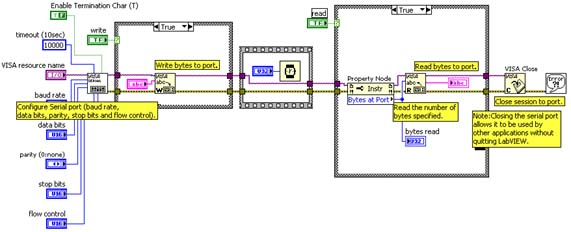
\includegraphics[height=6cm]{uart4}
\rule{30em}{0.5pt}
\caption{Write/Read a string to and from a COM port}
\label{fig:uart4}
\end{figure}
The VISA Configure Serial Port VI initializes the port identified by VISA resource name to the specified settings: timeout sets the timeout value for the serial communication; baud rate, data bits, parity, and flow control specify those specific serial port parameters.
\begin{enumerate}
\item The VISA Configure Serial Port VI initializes the port identified by VISA resource name to the specified settings: timeout sets the timeout value for the serial communication; baud rate, data bits, parity, and flow control specify those specific serial port parameters.
\item The VISA Write function sends the string.
\item The VISA Read function reads back up to bytes into the buffer, and the Simple Error Handler VI checks the error condition.
\item The VISA Close function terminates the communication channel to the instrument and deal locates the resources for the DSP.
\end{enumerate}
Depending on the purpose, the string can be written to the device in different forms. As the subVI described below, the string is combined by three parts, which are identified parameter order (two characters), the value needed to pass, and the character that uses for identifying read or write (character "w"). It is important to notice that maximum character transmission rate is depended on the baud rate and the bits per frame. More specifically, this rate is just the baud rate divided by the bits per frame. So, when there is a consecutive transfer required, the number of characters per string needs to be cared. Otherwise, there will be data lost.
\begin{figure}[htbp]
\centering
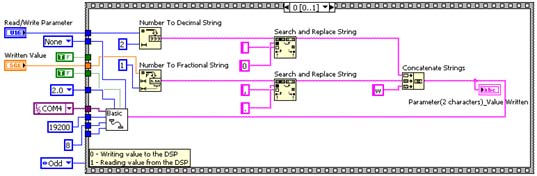
\includegraphics[height=4.8cm]{uart5}
\rule{30em}{0.5pt}
\caption{Formatting a string before writing to DSP}
\label{fig:uart5}
\end{figure}
Based on the prime subVI as showed in figure \ref{fig:uart5}, there are a number of ways to program an application that writes and reads multiple parameters to and from a DSP Processor. It needs to be reminded that, the principle of transferring data between DSP and PC is based on the interrupt. In other words, every time data is written to the DSP from PC, the serial DSP interrupt occurs and then its ISR (interrupt service routine) will run and process the received data. As a result, it is impossible to write more than one parameter at the same time that the DSP can process independently. Of course, each parameter has a different purpose. Because of this, the parameters should be organized so that only one parameter can write its data to the DSP at the time. It is very important for copying data between parameters that will be studied later.\\
Figure \ref{fig:uart6} shows an example program that wants to write multiple parameters to the DSP.\\
\begin{figure}[htbp]
\centering
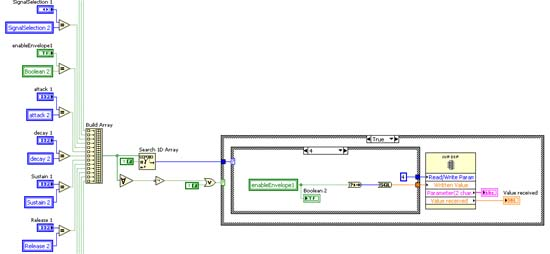
\includegraphics[height=6.6cm]{uart6}
\rule{30em}{0.5pt}
\caption{A part of writing parameters to Operator 1 program}
\label{fig:uart6}
\end{figure}\\
The idea of the program is that every time a parameter changes its value, which is detected due to search 1D array, the read/write part starts working. Otherwise, the program does nothing. This reduces a lot of works for the DSP Processor. Then, the latest value of the parameter and its order will be combined into string before writing to the processor. Notice that, LabVIEW also provides some data convert functions so that different data types of parameters can work properly.
%----------------------------------------------------------------------------------------
\subsection{UART Interrupt}
There are three things needed to be cared while using UART interrupts. First, you must map the UART interrupts to one of the interrupts in the interrupt vector table. In particular, the UART has to be mapped to exactly the peripheral interrupt sources. This can be achieved by changing the default source of the peripheral interrupt priority control register with the UART source, using the interrupt select values of the UART receive interrupt. The receive interrupt select values for UART0 (using in our application program) and UART1 are 0x13 and 0x14, respectively.
\begin{center}
\begin{tabular}[t]{|c|c|c|}
\hline
IIUART0RX & 0x3E00 & Internal Memory Address for UART0 Receiver\\
\hline
\end{tabular}
\end{center}
\begin{figure}[htbp]
\centering
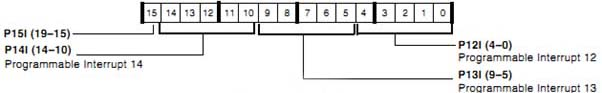
\includegraphics[height=1.5cm]{uart7}
\rule{30em}{0.5pt}
\caption{PICR2 Register}
\label{fig:uart7}
\end{figure}
\begin{alltt}
   *pPICR2 &= ~(0x3E0);  // Sets internal memory address for UART0 receiver
   *pPICR2 |= (0x13<<5); // Sets default value (0x13) for the URAT0 receive interrupt
\end{alltt}
The second thing is that enabling the UART interrupts internally by setting the corresponding bits in the UART interrupt enable register (UARTxIER). This needs to be done after all the UART settings (such as word length, parity, and so on) have been programmed, because in transmit mode as soon as the transmit buffer empty bit is enabled in the UARTxIER register, it vectors to the interrupt. If this bit is enabled before any of the UART settings are programmed, the data transmitted in the transmit interrupt service routine does not comply with the UART settings that are programmed later, leading to a communication error.
\begin{alltt}
   *pUART0IER = UARTRBFIE;   // Enables UART0 receive interrupt
\end{alltt}
The third, which is also the most important, is that using C Interrupt Handler with own Interrupt Service Routine. C provides its own set of interrupt handlers via the interrupt() and signal() functions. VisualDSP++ has extended the interrupt() function with \textbf{interruptf()} and \textbf{interrupts()} versions. The interrupt handler consists of three parts - the initialization, the interrupt vector, and the interrupt service routine. 
\begin{alltt}
   interrupt(SIG_P13, UARTisr);
\end{alltt}
Initialization performs the tasks previously associated with the C interrupt() function - assigning the interrupt service routine to an interrupt vector (dynamic ISR vectors only), unmasking the interrupt, and enabling global interrupts. The interrupt vector routes execution to the appropriate interrupt service routine. This routine must be compatible with the procedure of writing data of LabVIEW program. Otherwise, the data that DSP Processor expected to receive is different with data transmitted.
\begin{alltt}
   // Read the data from the buffer
   // Receive Buffer Registers (UARTxRBR)
      value = *pUART0RBR;
 
   /* Echoes back the value on to the hyperterminal*/
   // Wait until it is sent
      while ((*pUART0LSR & UARTTHRE) == 0)\{ ; \}

   // Writting a string to DSP
   // The character in buffer is "w" (ASC-II of "w" = 0x77 equivalent to 119 decimal)
      if(value == 119)
      \{
         for(i = 0; i < 2; i++)  address[i] = inputstream[i]; 
      
         // The two first characters writting from LabView is the index
         // int atoi(const char *str); - Convert string to integer 
            index = atoi(address);

         // The rest of the writting string is value (with a character - w)
         // Double atof ( const char * str ); - Convert string to double
         // 2 - is the place of starting value string 
            writtenValue = atof(inputstream + 2);

         // Writting value to the global variable
            algoparam[index] = writtenValue;    

         // Adds data to the buffer
         // Transmit Holding Registers (UARTxTHR)
            *pUART0THR = value;

            teller = 0;
      \}
\end{alltt}
%----------------------------------------------------------------------------------------
\subsection{The FM synthesizer application}
The application is programmed to provide two services. First, the program can write the values of parameters to the DSP so that DSP board can produce different sounds. Secondly, the LabVIEW User Interface also can show a number of features of the signal, such as the form of the envelope, frequency domain and the spectrogram.\\
To provide the features above, the application is programmed following a hierarchy as figure \ref{fig:uart8}.
\begin{figure}[htbp]
\centering
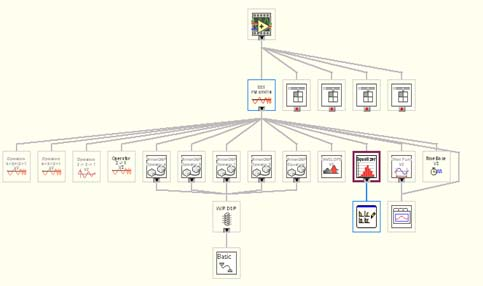
\includegraphics[height=5cm]{uart8}
\rule{30em}{0.5pt}
\caption{VI Hierarchy of LabVIEW User Interface}
\label{fig:uart8}
\end{figure}
\begin{figure}[htbp]
\centering
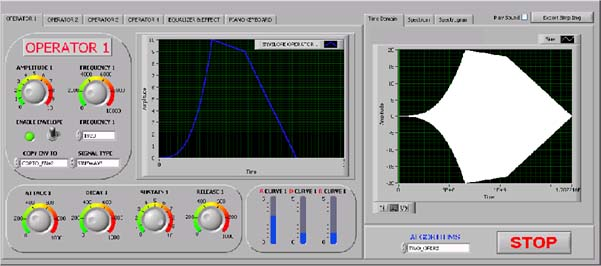
\includegraphics[height=5cm]{uart9}
\rule{30em}{0.5pt}
\caption{Front Panel of the application}
\label{fig:uart9}
\end{figure}
There are four main parts programmed in the application, which are programs for different algorithms of combining operators, programs for the envelope, programs for equalizer, sound effect and display, and writing data to the DSP board. The first part includes four algorithms: two operators, three operators, four operators modulated straightforward and four operators that actually consist of a pair of two operators. This part can be expanded in future to have more possibilities for producing sounds.
\begin{figure}[htbp]
\centering
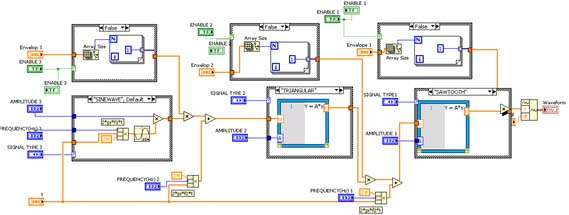
\includegraphics[height=5cm]{uart10}
\rule{30em}{0.5pt}
\caption{The algorithm for three operators}
\label{fig:uart10}
\end{figure}
The second part of the application is the envelope. It is used to modify the shape of the signal so that the output can have different frequency components. The third is programmed to produce more flexibility for the application. With this, user can choose specific range of frequency of the output signal (using the equalizer) and also can make distortion (using the effect part). The last one is writing data part, which is discussed in ''LabVIEW program for writing data", see section \ref{sec:Pham} above. More detail about the application, subVIs is available in appendix part in this report.
%----------------------------------------------------------------------------------------
\section{Conclusion}
This report discusses a number of things, which are needed to take into account when working with UART controller of the DSP processor and LabVIEW program. From my point of view, despite the fact that each part plays a different role to make the application work properly, the most important thing is that the data (a string of characters) need to be define completely the same in LabVIEW User Interface and UART interrupt service routine. Otherwise, the data that DSP Processor wants to receive for processing is not expected.\\ To improve quality of communication between LabVIEW User Interface and DSP board, context switch of UART interrupt needed to be considered. However, because of time and the limited ability, it could be studied in the future.
